\documentclass[10pt]{article}
\usepackage[margin=1in]{geometry}
\usepackage{graphicx}
\usepackage{booktabs}
\usepackage{array}
\usepackage{xcolor}
\usepackage{amsmath}
\usepackage[colorlinks=true,linkcolor=black,urlcolor=blue!50!black,citecolor=black]{hyperref}
\usepackage{caption}
\captionsetup{font=small,labelfont=bf}
\setlength{\parskip}{4pt}
\setlength{\parindent}{0pt}
\newcommand{\todo}[1]{\textcolor{red}{[#1]}}
\newcommand{\code}[1]{\texttt{#1}}

\title{CSC490 Assignment A4: RL-ing nanochat}
\author{}
\date{}

\begin{document}
\maketitle
\vspace{-2.2em}

\begin{center}
\begin{tabular}{ll}
\toprule
Team member & Student ID \\
\midrule
Allaith Ahmed Alzoubi & 1009064744 \\
Royce Luo & 1010192391 \\
Yujie Zeng & 1009321020 \\
Jinhao Zhang & 1008870839 \\
\bottomrule
\end{tabular}
\end{center}

\section*{Summary}
We ran nanochat's SFT, midtraining and reinforcement-learning scripts on our A3 model, a 24-layer Forgetting Transformer. Adding two math datasets raised GSM8K accuracy from 7.1\% to 20.3\% for SFT and from 5.1\% to 20.2\% for midtraining. A compute-matched SFT control reached only 7.4\%. The original RL run increased greedy GSM8K accuracy from 6.75\% to 14.71\%, but our analysis found that many incorrect responses stopped without producing a final answer.

We tested two additional rewards targeting answer completion and intermediate arithmetic. The completion reward performed best, reaching 19.18\% accuracy, while the arithmetic and combined rewards reached 15.16\% and 16.60\%. We then tested fixed-teacher on-policy distillation using the completion-reward model as the teacher. The main distilled model reached 8.79\%, while lower-learning-rate and shorter-rollout ablations improved to 13.72\% and 14.03\%. Neither surpassed the original RL baseline. Overall, encouraging complete answers was the most effective intervention we tested. Our conclusions are limited by single-run experiments, interrupted training sessions and differences between our model and Karpathy's original setup.
\section*{Part 1: nanochat's RL compared with GRPO}

nanochat's RL script, \code{chat\_rl.py}, is labeled GRPO, but its own docstring says it is closer to plain REINFORCE. In standard GRPO \cite{shao2024}, the model answers each question several times, and each answer is scored against the group's average and spread. The update is then kept in check in two ways: a limit on how far one update can move the model, and a penalty for drifting away from a frozen copy of the original model. nanochat removes both. It also scores answers against the group average only, without dividing by the spread, and it counts every token equally instead of averaging within each answer first. Karpathy may have made these changes to keep the code simple. Since nanochat uses each batch for only one on-policy update, PPO-style clipping is less necessary. Removing the frozen reference model also saves memory, although it removes an explicit constraint on policy drift. Counting every token equally follows DAPO \cite{yu2025dapo}, which found that averaging within each answer gives long answers less weight per token. Liu et al.\ \cite{liu2025} report a related length bias in GRPO. Dividing by the spread can also over-boost very easy and very hard questions when the score is just right or wrong, as it is here (for a fraction $p$ of right answers the spread is $\sqrt{p(1-p)}$, which is small when $p$ is near 0 or 1). The tradeoff is that nothing holds the model near where it started, so stability probably rests on small learning rates and a single pass over the data.

\footnotesize The assignment's reference list gives arXiv:2402.05191 for Shao et al.; that identifier belongs to an unrelated paper, and DeepSeekMath is arXiv:2402.03300. The claims about nanochat come from the docstring and code of \code{scripts/chat\_rl.py} at commit 92d63d4 (identical to master). The reasons for the changes are our inference.
\normalsize

\section*{Setup shared by Parts 2 and 3}

\textbf{Model.} Our starting point is the final A3 model, a 24-layer Forgetting Transformer (FoX \cite{fox}) checkpoint (step 5571). We chose our A3 model because the assignment is framed as continuing to train the model we built, so the results show what SFT, midtraining and RL add to a model we trained ourselves. The cost is that Karpathy's published numbers come from a different model (a depth-20 GPT), so our comparison with his run in Part 3 is not the exact same. Nanochat builds a standard GPT, so we load the checkpoint through a small wrapper that swaps in the FoX attention. nanochat's generation also needs a key/value cache, which the A3 attention did not support, so we added one (the cache stores keys, values and the running forget-gate sum; PR \#34) and checked that cached and uncached outputs match.

\textbf{Code.} nanochat is pinned at commit 92d63d4. Karpathy deleted the midtraining script on January 31, so we restored \code{mid\_train.py} from the commit before its removal. One edit was needed for a changed MMLU argument, and we removed a closing block that imported a module that does not exist at the pinned commit (that import crashed the first midtraining run while it was saving). Everything runs on Modal, on 8 GPUs per job (we asked for H100s, but Modal sometimes assigns an H200; see Part 2), and training is logged to Weights \& Biases.

\textbf{Scores.} We evaluate on the full test sets: all 1{,}319 GSM8K problems \cite{cobbe2021}, ARC-Easy, ARC-Challenge and MMLU, with greedy decoding. ChatCORE here means nanochat's centered mean over those four tasks (chance maps to zero); we leave HumanEval out.

\section*{Part 2: SFT and midtraining}

\subsection*{Original runs}
We ran both scripts from the pretrained model with nanochat's default settings, one run each. SFT trains only on the assistant's tokens; its mix is SmolTalk (460K chats), MMLU auxiliary train three times and GSM8K train four times, 789{,}759 rows in all. The midtraining script also trains on user tokens and adds identity conversations and spelling tasks. Table~\ref{tab:p2} gives the results, Figure~\ref{fig:p2} shows them, and Figure~\ref{fig:val} shows validation loss over training.

\begin{table}[h]
\centering
\small
\begin{tabular}{lrrrrrrr}
\toprule
Model & GSM8K & ARC-E & ARC-C & MMLU & ChatCORE & Steps & Val.\ bpb \\
\midrule
Pretrained & 0.0 & 24.9 & 22.7 & 22.9 & $-0.015$ & & \\
SFT & 7.05 & 25.1 & 22.9 & 22.9 & 0.004 & 466 & 0.450 $\to$ 0.280 \\
SFT + extra data & 20.32 & 59.8 & 48.1 & 36.0 & 0.281 & 492 & 0.450 $\to$ 0.279 \\
SFT + control rows & 7.43 & 45.7 & 35.6 & 33.2 & 0.150 & 492 & 0.450 $\to$ 0.279 \\
Midtraining & 5.08 & 49.0 & 39.2 & 34.4 & 0.172 & 815 & 0.528 $\to$ 0.353 \\
Midtraining + extra data & 20.24 & 48.7 & 38.4 & 34.8 & 0.207 & 866 & 0.528 $\to$ 0.353 \\
\bottomrule
\end{tabular}
\caption{Accuracy (\%) on the full test sets, greedy decoding. ``Control rows'' are 34{,}378 chat conversations already in the SFT mix, added to match the extra-data run's training time. Val.\ bpb is validation bits per byte at the first and last check (lower is better); the SFT and midtraining validation sets differ, so bpb is not comparable across the two scripts.}
\label{tab:p2}
\end{table}

\begin{figure}[h]
\centering
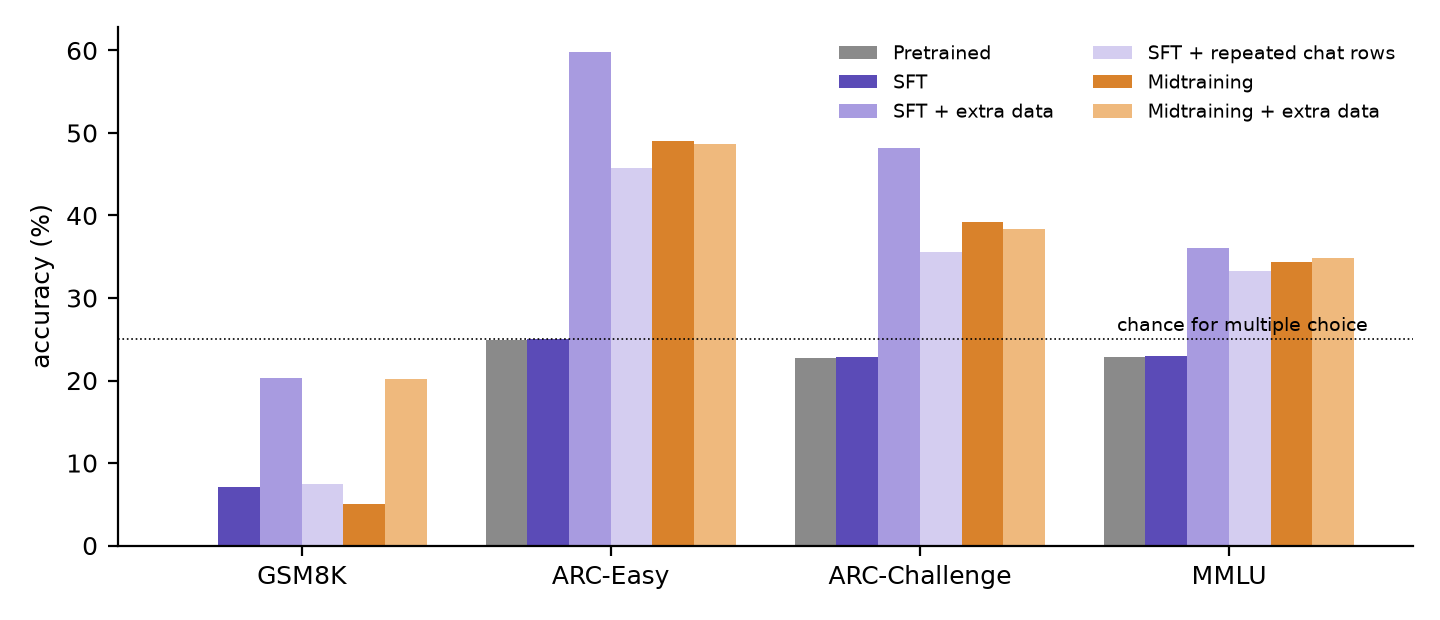
\includegraphics[width=0.78\textwidth]{figures/part2_scores.png}
\caption{Test accuracy of the six Part 2 models.}
\label{fig:p2}
\end{figure}

\begin{figure}[h]
\centering
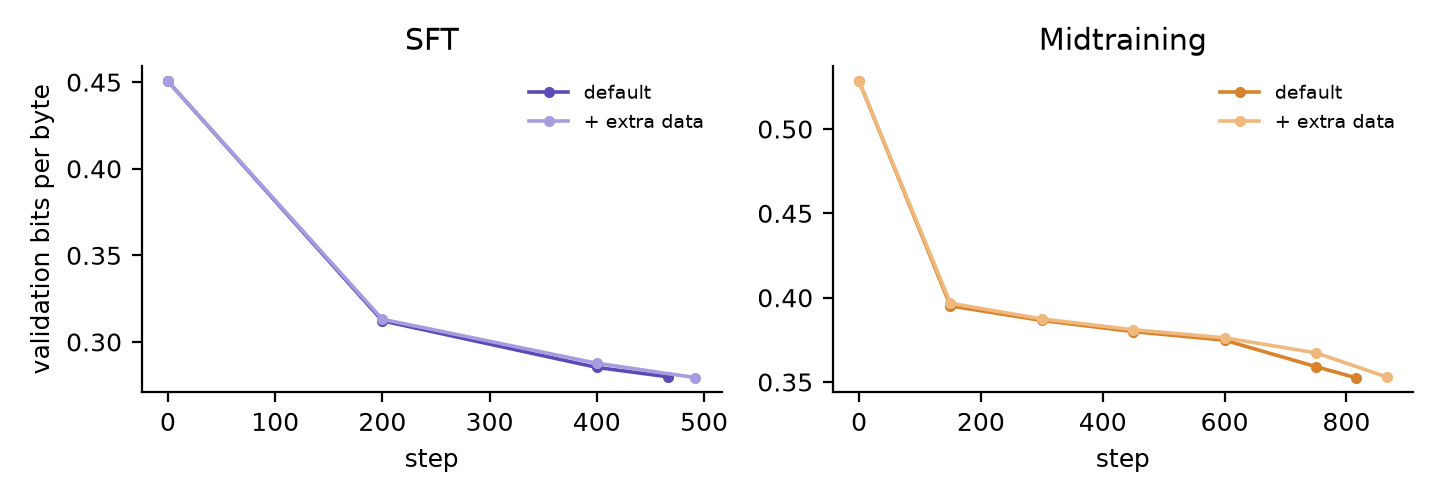
\includegraphics[width=0.85\textwidth]{figures/part2_validation.png}
\caption{Validation bits per byte at each check. It is almost the same with and without the extra data, because the validation sets are the default mixes, so this measure does not show the GSM8K gain.}
\label{fig:val}
\end{figure}

With 1{,}319 GSM8K problems, one standard error is about 0.7 points near 7\% and 1.1 points near 20\%. The jump from the original runs to the extra-data runs is many standard errors wide. The gap between the two original runs (7.05\% against 5.08\%) is about two standard errors.

\textbf{Default SFT fails on multiple choice.} Its MMLU score is exactly 3{,}222 of 14{,}042 correct, which is what answering ``A'' to every question gives (3{,}222 test answers are A). To see why, we looked at every fifth MMLU test question (2{,}809 of them; Table~\ref{tab:mc}). nanochat caps every output score at 15 (it computes $15\tanh(s/15)$). The default SFT model's scores for all four letters sit at that cap on every question, so the evaluation sees a four-way tie and picks the first letter. The other fine-tuned models' letter scores stay below the cap and differ from question to question, and they pick all four letters. The pretrained model also picks A 99\% of the time, but its scores are not capped (A 10.1 against 9.0 for B), so that is an ordinary bias. In the training log, the default SFT run's MMLU score was 25.0\% at step 200 and exactly the all-A value at steps 400 and 466, and a second default run shows the same value, so the failure appears during training. Our reading, which we did not prove, is that once the letter scores reach the cap the gradient through the cap is close to zero, so the model cannot move back out. Midtraining, which uses the same multiple-choice data, did not saturate (ARC-Easy 49\%).

\begin{table}[h]
\centering
\small
\begin{tabular}{lrrr}
\toprule
Model & Letter chosen A/B/C/D (\%) & Mean score A/B/C/D & Accuracy (\%) \\
\midrule
Pretrained & 99.0 / 0.7 / 0.0 / 0.3 & 10.1 / 9.0 / 8.6 / 8.8 & 24.0 \\
SFT & 100 / 0 / 0 / 0 & 15.0 / 15.0 / 15.0 / 15.0 & 24.0 \\
SFT, different data order & 99.7 / 0 / 0 / 0.3 & 15.0 / 15.0 / 15.0 / 15.0 & 24.0 \\
SFT, rerun on an H100 & 0 / 0 / 0 / 100 & 15.0 / 15.0 / 15.0 / 15.0 & 27.0 \\
SFT + control rows & 18.1 / 18.0 / 43.0 / 20.9 & 14.0 / 13.9 / 14.1 / 13.9 & 32.1 \\
SFT + extra data & 21.5 / 26.6 / 33.5 / 18.4 & 12.2 / 12.3 / 12.4 / 12.1 & 34.3 \\
Midtraining & 26.3 / 22.5 / 24.6 / 26.6 & 13.5 / 13.4 / 13.5 / 13.5 & 34.4 \\
\bottomrule
\end{tabular}
\caption{What each model does on 2{,}809 MMLU test questions (every fifth). The correct letters are A 24.0\%, B 25.2\%, C 23.8\%, D 27.0\%. The score is nanochat's capped output score (maximum 15) for each answer letter. The four SFT rows were scored on an H100; the pretrained and midtraining rows were scored earlier on a GPU that was not recorded.}
\label{tab:mc}
\end{table}

\subsection*{Extra datasets}
\textbf{Choice.} Our target metric is GSM8K, so we chose two grade-school math sets that are close to it and that can be written in the format nanochat's grader reads (a final line \code{\#\#\#\# N}).
\begin{itemize}
\item \textbf{MetaMathQA} \cite{metamath} has 395{,}000 rows and an MIT license. Its dataset card says all of it is augmented from the training sets of GSM8K and MATH, and that none of it comes from the test sets. We use the 40{,}000 \code{GSM\_AnsAug} rows (new solutions to GSM8K questions) and 40{,}000 \code{GSM\_Rephrased} rows (reworded questions). Its answers end with \code{\#\#\#\# N} followed by a line ``The answer is: N'', which we remove.
\item \textbf{Orca-Math 200K} \cite{orcamath} has 200{,}035 rows and an MIT license. According to its card, the questions were expanded from seed sets (Lila and DMath) with GPT-4 Turbo, which also wrote the answers. We use 40{,}000 rows. Its answers are prose without a marker, so we kept the rows whose last number falls within the final 40 characters of the answer and appended \code{\#\#\#\# N} with that number.
\end{itemize}
Orca-Math adds problems from different sources than GSM8K, and MetaMathQA adds new solutions in GSM8K's own style. We did not run the two datasets separately, so we cannot say how much each contributes, and each configuration is a single run.

\textbf{Same configuration.} The extra file (120{,}000 rows) is appended to the training mix of each script, which is otherwise unchanged. The mixes grow from 789{,}759 to 909{,}759 rows for SFT, so the extra-data runs take more steps (492 against 466 for SFT, 866 against 815 for midtraining). For SFT, we address this with a compute-matched control using repeated examples from the original training mix, described below. We did not run an equivalent control for midtraining, so some of its improvement could come from additional training.

\textbf{Overlap with the test set.} We dropped any candidate that shares a 13-word span (numbers blanked) with a GSM8K test question; this removed 97 candidates. An afterwards check found no exact test question in the final file. A separate n-gram comparison of the file found 22 rows that share a 12-word span with a test question and 416 that share a 10-word span; we have not removed them, and we think the effect is small but did not measure it.

\textbf{Repetition.} The final file has 78{,}320 distinct questions in 120{,}000 rows, and 41{,}431 of the rows (7{,}140 distinct questions) are GSM8K \emph{training} questions that are already in the SFT mix. So part of the extra data is new answers to questions the model has already seen.

\subsection*{Results}
The extra data raised GSM8K accuracy to 20.3\% for SFT and 20.2\% for midtraining. For midtraining, nothing else moved by more than about a point (ARC-Easy 49.0\% to 48.7\%, MMLU 34.4\% to 34.8\%, ARC-Challenge 39.2\% to 38.4\%), which is the pattern one would expect from math-only data. For SFT, the multiple-choice scores jumped as well (ARC-Easy 25\% to 60\%). We do not credit that jump to the data: math problems should not teach multiple choice, midtraining did not show it, and the baseline it is compared with is the run whose scores saturated. We therefore use two baselines. On GSM8K, which is the target of the assignment, the default (7.05\%) and the control (7.43\%) agree, so that comparison does not depend on which one is used. On ARC and MMLU we treat the control as the fairer SFT reference, because the default run's scores are saturated.

\textbf{Controls and hardware.} Four further runs test whether this failure comes from the default settings. (1)~A compute-matched control uses the default settings and mix plus 34{,}378 chat conversations that are already in the mix (27{,}074{,}428 tokens counted with nanochat's renderer, against 27{,}073{,}584 for the math file), so it trains for the same 492 steps with no new information. On GSM8K it reaches 7.4\%, against 7.1\% for the default and 20.3\% for the math run, so the extra steps alone do not explain the GSM8K gain (one standard error is about 0.7 points). On multiple choice it reaches ARC-Easy 45.7\%, ARC-Challenge 35.6\% and MMLU 33.2\%, against 25\%, 23\% and 23\% for the default, and its letter scores are close to the cap (about 14.0) but do not tie (Table~\ref{tab:mc}). The math run is still higher on ARC (59.8\% and 48.1\%) while the two are close on MMLU (36.0\% against 33.2\%); with a single run of each, we cannot tell whether the remaining ARC gap comes from the math data or from run-to-run variation. (2)~The default mix with a different data order (shuffle seed 1) saturated as well: it chose A on 2{,}800 of 2{,}809 questions, with letter scores of 14.98 to 15.0. So the failure does not depend on the order of the data. (3)~A hardware check. Modal may substitute an H200 for an H100. The W\&B records show that the first three runs of the plain default mix trained on an H200, as did the control, while the math run trained on an H100 (the two midtraining runs and the final RL run also trained on H100s). Scoring the default model on a guaranteed H100 gives the same saturation (Table~\ref{tab:mc}), so the weights are saturated and the scoring GPU is not the cause. The control also trained on an H200 and did not saturate, so an H200 alone does not cause it. Finally, we reran the default settings pinned to an H100 (W\&B confirms the GPU, with the same data order as the first run): it saturated as well. It chose D on all 2{,}809 questions, with letter scores of 14.95 to 15.0, and its MMLU count at step 400 was 3{,}776 of 14{,}042, the number that answering D to every question gives. So four runs of the plain default mix saturated, three on an H200 and one on an H100, and the two runs with extra rows did not. The failure belongs to the default mix and settings on our model, not to the GPU. We do not know why the default mix fails while a mix with extra rows does not. We did not run a matching control for midtraining; its multiple-choice scores did not change with the extra data, so the comparison there does not show the same problem.

\section*{Part 3: RL replication}

\subsection*{Setup}
We ran \code{chat\_rl.py} with its default settings, starting from the default SFT model (the one whose multiple-choice scores saturate, see Part 2): 467 steps (one pass over the 7{,}473 GSM8K training problems at 16 problems per step), 16 sampled answers per problem, temperature 1, at most 256 new tokens, top-$k$ 50, and an evaluation every 60 steps on 400 test problems. Karpathy's post says he used the script's default settings and that they take about 1.5 hours. We added one thing to the script: a switch that saves every sampled answer with its reward, which the original discards (Part 3 asks us to review the answers during training).

\textbf{Attempts.} Modal can preempt GPU jobs. We made five RL attempts (Table~\ref{tab:attempts}); only the last reached step 467, and it did so by resuming a run that had been preempted. The run reported here is that run: steps 0 to 60 are in the Weights \& Biases run \code{a4-rl3} and steps 61 to 466 in \code{a4-rl3-resume}. Because nanochat does not save the optimizer state, the resumed run starts with a fresh optimizer. We therefore replicate the training procedure and total number of steps, but not the exact optimizer trajectory of an uninterrupted run. We show the first attempt as a second curve in Figure~\ref{fig:curves}.

\begin{table}[h]
\centering
\small
\begin{tabular}{lll}
\toprule
Attempt & What happened & Used for \\
\midrule
\code{a4-rl} & cancelled by Modal at step 316 & step-300 checkpoint; the second curve \\
\code{a4-rl2} & preempted at about step 300 & one evaluation (noise estimate) \\
\code{a4-rl2-resume} & resumed from step 300, stopped by us & nothing \\
\code{a4-rl3} & preempted after step 61 & steps 0 to 60 of the final run \\
\code{a4-rl3-resume} & resumed from step 60, ran to step 466 & steps 61 to 466; the final model \\
\bottomrule
\end{tabular}
\caption{The five RL attempts.}
\label{tab:attempts}
\end{table}

\subsection*{Comparison with Karpathy's run}
Karpathy published his RL run as final scores in two posts and as one chart image in his announcement post \cite{nanochat}; we found no public Weights \& Biases run or data file. His chart (for the depth-20 model) has three panels: training reward, pass@1 and pass@8. We read approximate values off the image (to about $\pm$0.002), so the comparison below is by eye. His pass@8 panel is plotted against minutes, not steps. It has eight points, and nanochat evaluates every 60 steps by default, so we place them at steps 0 to 420 in Figure~\ref{fig:curves}; that placement is our inference, and the pass@8 comparison is weaker than the other two panels. The assignment's reference list points to a different post (a pretraining post), so we used the RL section of the announcement post.

\begin{figure}[h]
\centering
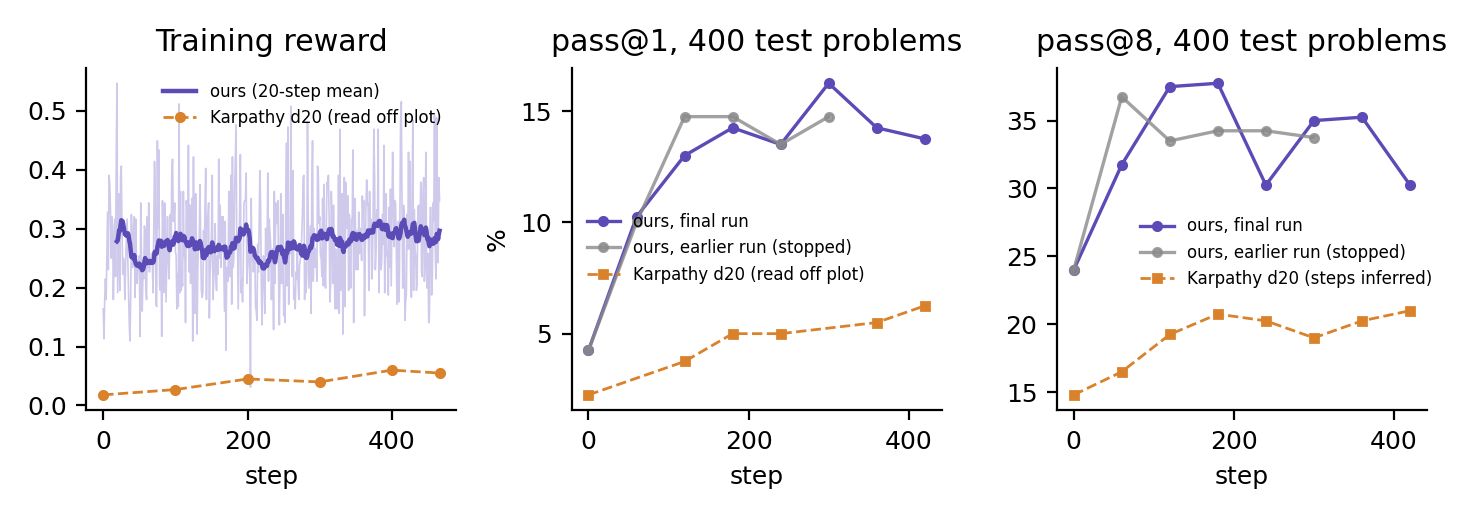
\includegraphics[width=\textwidth]{figures/part3_curves.png}
\caption{RL curves. Left: mean training reward per step (ours: 16 problems $\times$ 16 samples per step). Middle and right: pass@$k$ on 400 test problems at temperature 1. Karpathy's values are read off the chart in his announcement post. His pass@8 panel is plotted against minutes; its eight points are placed at steps 0, 60, \ldots, 420, which assumes the default evaluation interval of 60 steps (our inference, not read from the chart).}
\label{fig:curves}
\end{figure}

\begin{table}[h]
\centering
\small
\begin{tabular}{lrrr}
\toprule
& SFT model & After RL & Source \\
\midrule
Karpathy, depth 20 & 4.55 & 7.58 & announcement post \\
Karpathy, depth 32 & 12.74 & 19.94 & second post \\
Ours (full test set, greedy) & 6.75 & 14.71 & our answers \\
\bottomrule
\end{tabular}
\caption{GSM8K test accuracy (\%) before and after RL. Our SFT figure from the answer-dump script (89 of 1{,}319) differs from the 7.05\% in Table~\ref{tab:p2} (93 of 1{,}319) by four problems. Both use greedy decoding, but greedy decoding on a GPU is not exactly repeatable: running the answer-dump script twice on the same model changed 4 of the first 300 outcomes (and 113 of 300 answer texts), so a gap of this size is within run-to-run variation.}
\label{tab:karpathy}
\end{table}

\textbf{Differences.} Our model starts higher and ends higher than his depth-20 model: pass@1 on the 400-problem evaluation goes from 4.25\% to 13.75--16.25\% (his: 2.25\% to 6.25\%), and our mean training reward is about 0.28 against his 0.02 to 0.055. The shape differs too. Our reward jumps from 0.16 at step 0 to about 0.28 within the first 20 steps and then stays within a few hundredths, while his rises slowly through the run. After step 120 our pass@1 moves around between 13\% and 16\% with no clear trend. On pass@8 our model starts at 24.0\% and stays between 30.2\% and 37.8\% for the rest of the run, again with no clear trend, while his goes from about 14.8\% to about 21.0\%. Our training reward at step 0 (0.164) is about four times our test pass@1 (0.0425), while Karpathy's two numbers are about equal (0.018 and 0.0225). The SFT mix includes the GSM8K training problems four times for both models, so we do not know why our gap is larger; memorized training solutions are one candidate we did not test.

We can list likely causes, but we did not test any of them. (1)~Different starting models: ours is a depth-24 Forgetting Transformer from A3, his is a depth-20 GPT, and our SFT model is already stronger on GSM8K (7.05\% against 4.55\%) and also gains more from RL (about 8 points against 3). (2)~Different pipelines: his SFT follows midtraining, ours is run directly from the pretrained model. (3)~Noise: three runs of the same setting gave pass@1 of 14.75\% (first attempt), 14.25\% (second, the W\&B run \code{a4-rl2}) and 16.25\% (final run) at step 300, so a spread of about two points is normal on 400 problems; our final model's 14.7\% on the full test set is also below the 16.4\% of the first run's step-300 model, within that spread. (4)~We did not control for any of these, so we cannot say which matters.

\textbf{Where the early gain comes from.} Most of the first jump in training reward is the model learning to finish its answers: from step 0 to the first 20 steps, the share of sampled answers with a final line rises from 68\% to 88\%, and the accuracy among answers with a final line rises from 24\% to 32\%. Later the two move apart. Accuracy among answers with a final line keeps rising (36\% in steps 200 to 349, 42\% in steps 350 to 466, 45\% in the last 20 steps) while the share with a final line falls, so the gain after the first 20 steps comes from more accurate finished answers, not from finishing more often.

\subsection*{What the model gets right and wrong}
We saved all 119{,}552 answers the model sampled during training (7{,}472 problems, 16 each, steps 0 to 466, each with its reward) and the greedy test answers of the SFT model and the final RL model.

\textbf{Which problems.} Of the 7{,}472 training problems, 2{,}815 (38\%) were never solved in 16 samples, 4{,}306 (58\%) were solved sometimes and 351 (5\%) always. Reward falls with question length (0.44 under 30 words, 0.30 for 30--49, 0.16 for 50--79, 0.09 for 80 or more) and with the number of numbers in the question (0.34 for 0--1, 0.32 for 2--3, 0.22 for 4--5, 0.14 for 6 or more). We also clustered the questions by their words (TF-IDF and $k$-means with $k=8$). The hardest clusters were age problems (reward 0.22, 205 questions) and speed and time problems (0.23, 530); the easiest were counting-items problems (0.30, 763). Mean reward varies less across the topic clusters (0.22 to 0.30) than across the question-length groups (0.09 to 0.44). One cluster, made of generic words such as number, total and times, holds 53\% of the problems, so the clustering separates only a few distinct topics. The SFT model has also already trained on these problems (four passes over the GSM8K training set), so these counts describe problems it has seen.

\textbf{Why answers are wrong.} We labeled every wrong training answer with rules we wrote, applied in a fixed order (Figure~\ref{fig:fail}, Table~\ref{tab:fail}). The labels describe what an answer looks like, not necessarily the cause; for instance, ``off by a whole factor'' only says the result is a multiple or fraction of the right one. To find out how far the rules can be trusted, we drew a stratified sample of 100 wrong training answers (10 per rule label for eight of the wrong-answer labels, and 20 without a final answer) and had a separate language-model reader label each one, without seeing the rule labels, using its own list of reasons (misread relation, missing quantity or step, percent or ratio mistake, incoherent steps, and so on). This is a model's judgment, not a person's, and the sample is small. Where a rule implies a specific reason, the reader agreed on 33 of 60 items (55\%). It agreed on the calculator-call cut-offs (4 of 4) and digit loops (3 of 4), but on only 4 of 10 for ``never uses a number the question gives'' and ``right value, then reports another'', and on 5 of 10 for ``uses a number found nowhere''. The rules for ``off by a whole factor'', ``off by 1 or 2'' and ``repeats a number'' describe the result and not the reason: the reader spread each of them over five or six different reasons. So we treat the rule labels as descriptions of how an answer looks, and use the reader's labels for the reasons.

\begin{figure}[h]
\centering
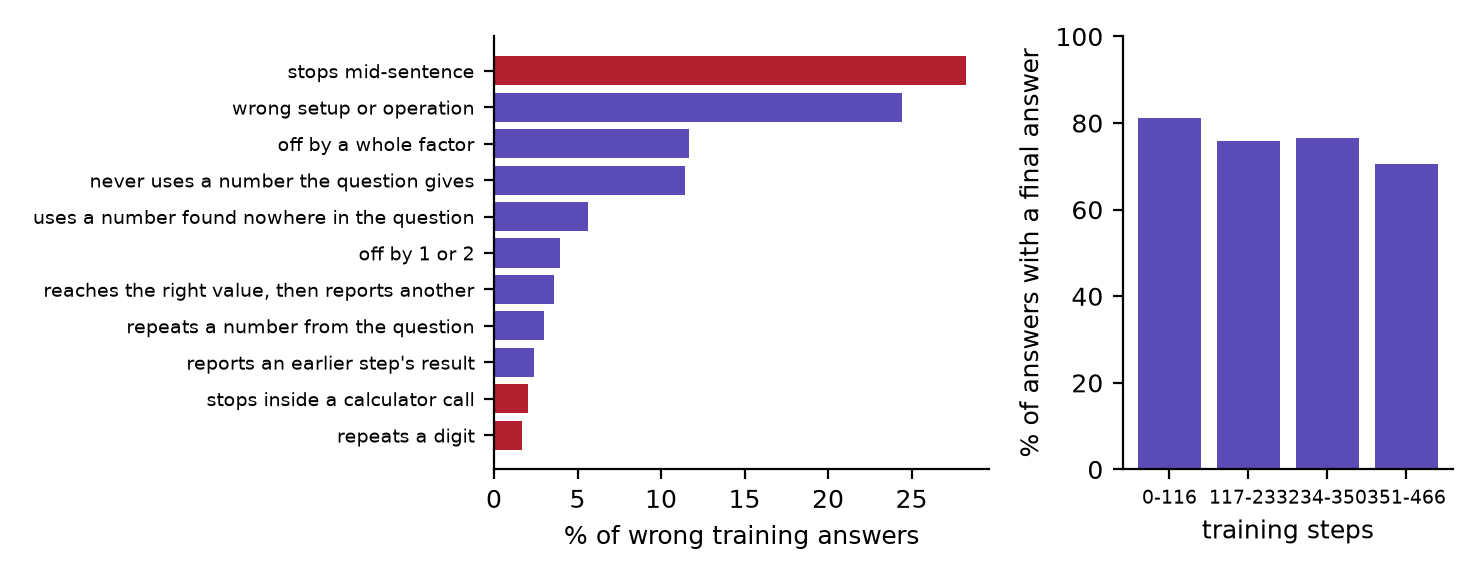
\includegraphics[width=0.95\textwidth]{figures/part3_failures.png}
\caption{Left: kinds of wrong answer during training (red: no final answer). Right: share of sampled answers that contain a final answer, by stage of training.}
\label{fig:fail}
\end{figure}

\begin{table}[h]
\centering
\small
\begin{tabular}{lrr}
\toprule
Kind of wrong answer & Training & Test, final model \\
\midrule
No final answer (all kinds) & 33.1\% & 39.8\% \\
\quad stops mid-sentence & 28.2\% & 34.8\% \\
\quad stops inside a calculator call & 2.1\% & 1.0\% \\
\quad repeats a digit & 1.7\% & 2.6\% \\
\quad stops after a full sentence & 1.1\% & 1.4\% \\
Wrong final answer (all kinds) & 66.9\% & 60.2\% \\
\quad wrong setup or operation, all numbers present & 24.4\% & 23.2\% \\
\quad off by a whole factor & 11.7\% & 10.4\% \\
\quad never uses a number the question gives & 11.4\% & 11.2\% \\
\quad uses a number found nowhere in the question & 5.7\% & 3.2\% \\
\quad off by 1 or 2 & 3.9\% & 3.5\% \\
\quad reaches the right value, then reports another & 3.6\% & 4.4\% \\
\quad repeats a number from the question & 3.0\% & 2.9\% \\
\quad reports an earlier step's result & 2.4\% & 1.3\% \\
\bottomrule
\end{tabular}
\caption{Share of wrong answers by label. Training: 86{,}569 wrong answers (sampled, temperature 1, 256-token limit). Test: 1{,}125 wrong answers of the final model (greedy, 512 tokens). Small categories are omitted.}
\label{tab:fail}
\end{table}

Weighting the reader's labels by how common each rule label is, the estimated reasons among the wrong answers that do give a final answer are shown in Table~\ref{tab:reasons}. Examples: using the wrong operation (subtracting where it should multiply), applying a percentage backwards (answering 384 to a 20\% discount problem with a final price of \$480, reference 600), skipping a quantity the question gives (ignoring ``12 rings per pineapple''), or writing steps that do not follow from each other. Because each interval comes from 10 labeled answers per rule label, the intervals are wide, and a reader could reasonably move an answer between neighboring reasons (the reader rated 45 of its 100 labels medium confidence and 3 low).

\begin{table}[h]
\centering
\small
\begin{tabular}{lrr}
\toprule
Reason (reader's label) & Estimated share & 95\% interval \\
\midrule
Misread how the quantities relate & 26\% & 14--39\% \\
Incoherent steps or invented numbers & 25\% & 15--36\% \\
Missing quantity or step & 21\% & 11--32\% \\
Percent, fraction or ratio mistake & 15\% & 5--26\% \\
Wrong operation & 7\% & 0--16\% \\
Extra step, unit conversion, misreported answer, other & 6\% & \\
\bottomrule
\end{tabular}
\caption{Estimated reasons for the 57{,}210 wrong training answers covered by the eight wrong-answer labels (of 57{,}938 that give a final answer), from the 80 labeled items weighted by rule-label frequency (bootstrap intervals).}
\label{tab:reasons}
\end{table}

\textbf{Answers that never finish.} About a third of wrong training answers, and 40\% of wrong test answers, stop without a final \code{\#\#\#\# N} line. We checked that this is the model's own behavior and not a bug in our cache: we replayed 40 such answers from the first RL run and ran the same tokens through the plain forward pass with no cache, which also predicts the end-of-turn token at the stopping point in 36 of the 40 cases (three of the 40 were digit loops that ran to the limit). Training data does not teach this. In the GSM8K training set the turn never ends within five tokens of the last calculator result, and every example ends with a final answer line. The reader judged that among answers without a final line about 52\% are cut off midway and 44\% reach the end of a thought, often stating the answer in words, but never write the \code{\#\#\#\# N} line (4\% loop on a digit), so our ``stops mid-sentence'' label overstates how many are cut off. We do not know why the model stops; a small, partly under-trained model with a weak sense of when it is finished is one candidate, and we did not test it.

RL did not reduce this behavior on the final model. On the test set, 465 of the SFT model's 1{,}230 wrong answers (38\%) have no final answer and 448 of the final model's 1{,}125 (40\%) do. The kind changes: SFT often writes a full sentence with the answer in prose and no marker (413 cases; only 18 of its 465 answers without a marker end on the correct number), while the RL model more often is cut off mid-sentence (392). During training the share of sampled answers with a final line first rose, from 68\% at step 0 to 88\% over the first 20 steps, and then drifted down to 76\% (steps 200 to 349), 71\% (350 to 466) and 66\% (the last 20 steps) (Figure~\ref{fig:fail}, right). The 256-token limit is not the main cause: in a random sample of 15{,}000 training answers without a final line, only 4.5\% are 250 tokens or longer, and the median length is 56 tokens.

\textbf{SFT against RL on the test set.} The final RL model solves 194 of 1{,}319 problems and the SFT model 89. RL fixed 145 problems and broke 40; 49 are right in both and 1{,}085 in neither.

\section*{Part 4: Additional RL rewards}

\subsection*{Motivation and reward design}
Part 3 found that 33.1\% of the wrong answers sampled during RL training lacked a final answer, and 2{,}815 of 7{,}472 training problems were never solved in 16 samples. Both patterns are problems for a binary correctness reward: an answer that performs some correct intermediate work but gives the wrong final number receives the same zero as an answer that stops immediately, and a group with 16 wrong answers has zero group-centered advantage throughout. We added two small rewards to distinguish these cases. We kept nanochat's original binary correctness reward $R_c$ and the same group-centered policy-gradient update.

\textbf{A: Final-answer completion.} The first reward adds 0.15 when a response ends with exactly one valid \code{\#\#\#\# N} line, with $N$ a signed integer or decimal. It does not check whether $N$ is right. If $F(y)$ is one for a valid final line and zero otherwise, the reward is
\[
R_A(y)=R_c(y)+0.15F(y).
\]
This targets the premature stopping and missing-marker behavior in Part 3, without giving an incorrect but well-formatted answer as much reward as a correct one.

\textbf{B1: Verified intermediate arithmetic.} The second reward extracts arithmetic expressions and their results from the \code{<<expression=result>>} annotations in GSM8K's reference solutions. It checks that the operations are valid and the claimed numerical result is correct. It then searches the model's answer for matching calculations, including calculator calls. Matching is intentionally strict: expressions must have the same parsed operation structure, not merely equivalent numerical values. Let $G$ be the set of distinct, valid annotated reference calculations and $P(y)$ the corresponding set extracted from response $y$. We use
\[
A(y)=
\begin{cases}
|G\cap P(y)|/|G|,& |G|>0,\\
0,& |G|=0,
\end{cases}
\qquad
R_B(y)=R_c(y)+0.20A(y).
\]
The set-based score avoids rewarding repeated copies of the same calculation. It also gives no extra credit for calculations not found in the reference, even if they are mathematically valid; this is a limitation of the reward, not evidence that those steps are wrong.

\textbf{Combined reward.} We also trained a model with both terms:
\[
R_{A+B}(y)=R_c(y)+0.15F(y)+0.20A(y).
\]
The 0.15 and 0.20 weights are exploratory choices, not tuned optima. Together the bonuses cannot exceed 0.35, whereas a correct final answer earns at least 1. The three modes correspond to PRs \#41--\#43.

\subsection*{Setup}
We trained three separate models from the same default SFT checkpoint (step 466), rather than continuing from the Part 3 RL checkpoint. Each used the original RL configuration: one epoch of GSM8K, 467 optimizer updates, 16 problems per update, 16 sampled completions per problem, temperature 1, top-$k$ 50, and at most 256 new tokens. The learning rates and optimizer were unchanged. Evaluation during training used 400 GSM8K test questions, eight sampled answers per question, every 60 updates. We used eight H100 GPUs for each run, saved the final step-466 checkpoints, and recorded the curves in Weights \& Biases.

The original correctness-only result is the Part 3 run, not a new uninterrupted control: it was resumed after preemption without its optimizer state. The three new models were trained independently with matched settings, but each configuration was run only once. For the final comparison, we generated greedy answers with a 512-token limit for all 1{,}319 GSM8K test questions. The final scoring uses only the dataset's binary answer check, never the added rewards.

\subsection*{Results}
Table~\ref{tab:p4} reports the held-out accuracy. Completion-only performs best, solving 253 problems (19.18\%), against 194 (14.71\%) for the historical correctness-only RL model. Arithmetic-only solves 200 (15.16\%), a small gain over that historical baseline, while combining both rewards solves 219 (16.60\%). Adding arithmetic credit to completion credit therefore did not improve on completion alone.

\begin{table}[h]
\centering
\small
\begin{tabular}{lrrr}
\toprule
Model & Correct / 1{,}319 & Accuracy (\%) & Change vs.\ original RL \\
\midrule
Default SFT & 89 & 6.75 & $-7.96$ pp \\
Original RL (Part 3) & 194 & 14.71 & -- \\
Completion (A) & \textbf{253} & \textbf{19.18} & \textbf{$+4.47$ pp} \\
Arithmetic (B1) & 200 & 15.16 & $+0.45$ pp \\
Combined (A+B1) & 219 & 16.60 & $+1.90$ pp \\
\bottomrule
\end{tabular}
\caption{Greedy GSM8K test accuracy on 1{,}319 questions (512-token limit). Original RL is the historical Part 3 result; the other four models were evaluated in one answer-dump job. The historical run was resumed without optimizer state, so the differences against it are not a fully controlled comparison.}
\label{tab:p4}
\end{table}

\begin{figure}[h]
\centering
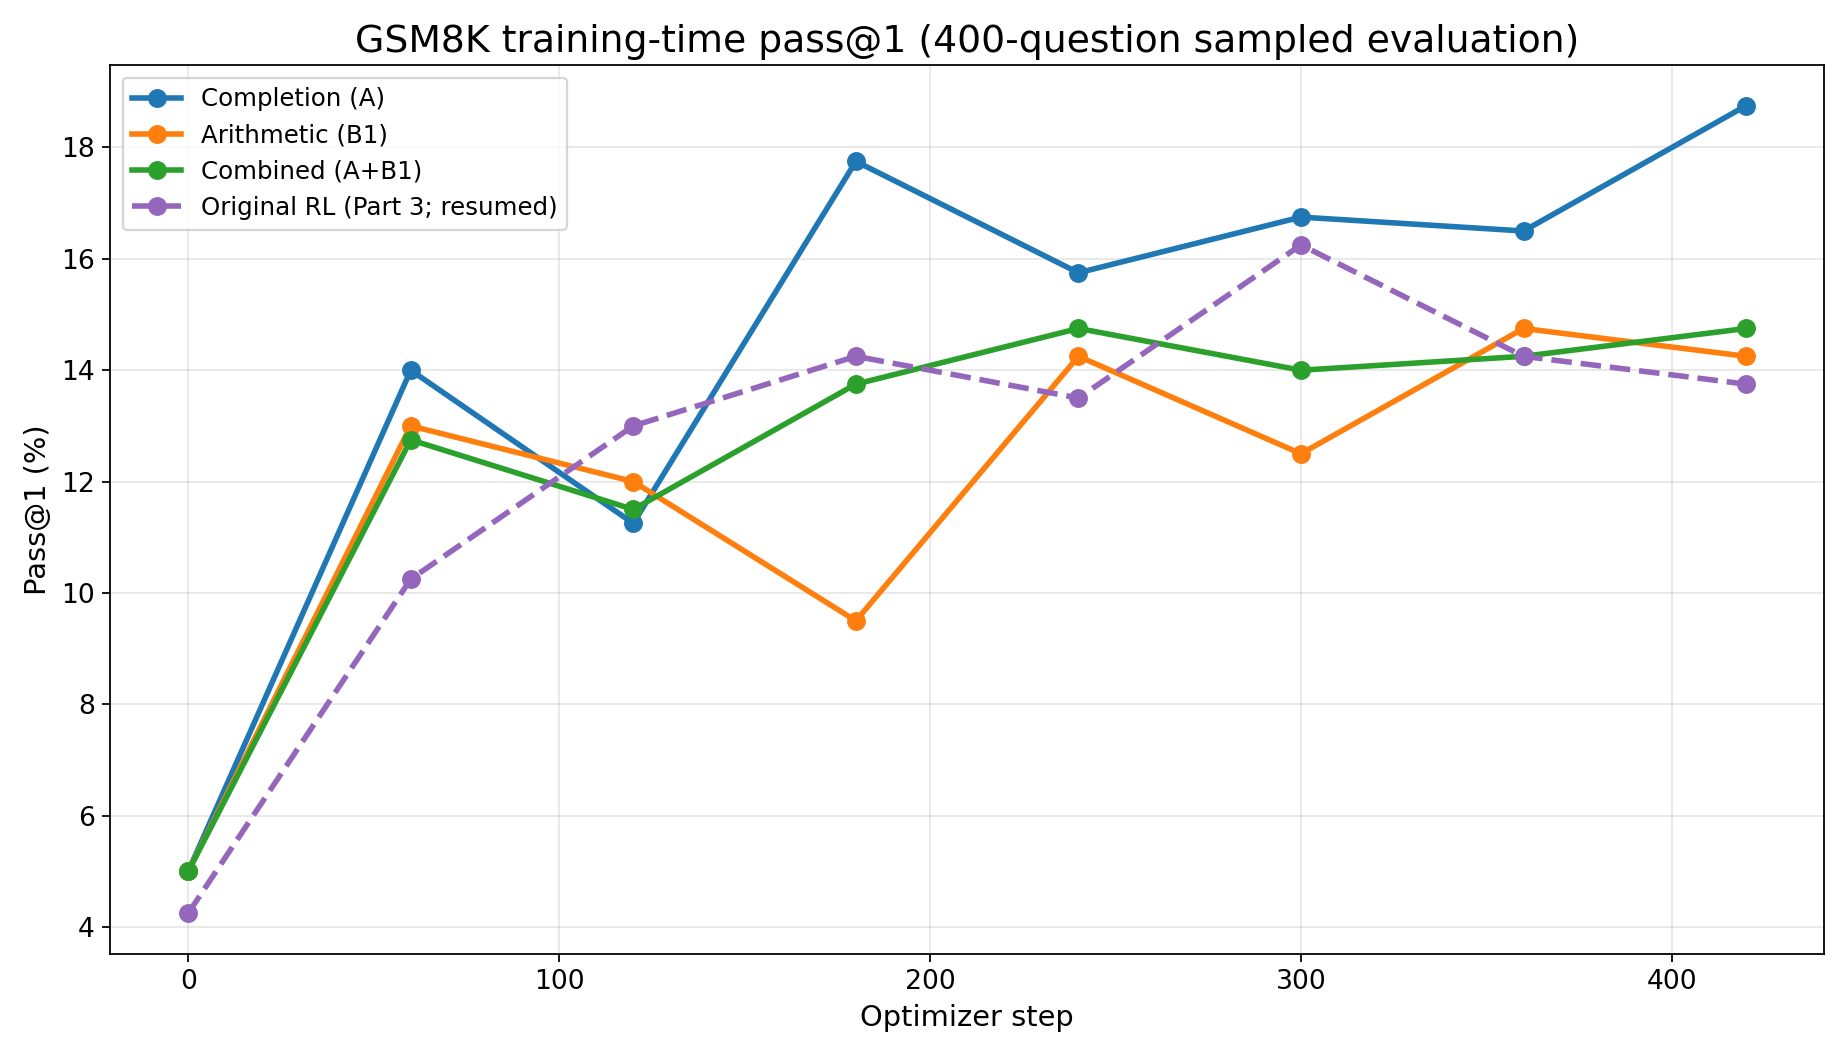
\includegraphics[width=0.82\textwidth]{figures/p4_pass1.png}
\caption{Pass@1 on 400 GSM8K test questions at temperature 1 for the original correctness-only RL run and the three additional reward configurations. Evaluations are shown every 60 training steps. The original run was interrupted and resumed without optimizer state, so the comparison is descriptive rather than fully controlled.}
\label{fig:p4_curves}
\end{figure}

The training-time evaluations agree with the held-out ranking (Figure~\ref{fig:p4_curves}). The final logged pass@1 is 18.75\% for completion, 14.25\% for arithmetic and 14.75\% for combined. The corresponding pass@8 values are 33.00\%, 32.50\% and 32.25\%. These evaluations use sampled decoding and only 400 questions, so their values should not be read as the final greedy test scores. The combined run also reaches the highest total training reward (about 0.675 at the last logged update, against 0.598 for completion and 0.560 for arithmetic), but its test accuracy is lower than completion-only. The total shaped reward is not directly comparable between methods because its definition differs.

\textbf{Paired differences.} We matched the four newly evaluated models by question index. Completion-only solves 116 questions that arithmetic-only misses, while arithmetic-only solves 63 that completion misses. Against combined, completion fixes 117 questions and loses 83. The respective accuracy gaps are 4.02 percentage points (paired bootstrap 95\% interval 2.05--5.99) and 2.58 points (0.53--4.70), based on 20{,}000 resamples of test questions. These intervals capture question-level variation, not variation across independent training seeds. We cannot make the same paired calculation against the historical RL model from the current four answer files.

\subsection*{What errors changed}
We categorized the held-out answers by whether they were correct, had a well-formed but wrong final line, had a malformed final line, or had no \code{\#\#\#\#} marker. These are observable properties, not explanations of the underlying reasoning error; a well-formed but wrong number could come from an incorrect setup, arithmetic or a missing step.


\begin{table}[htbp]
\centering
\small
\begin{tabular}{lrrrr}
\toprule
Model & Correct & Valid but wrong & Malformed & No marker \\
\midrule
Default SFT & 89 & 642 & 123 & 465 \\
Original RL (Part 3) & 194 & \multicolumn{2}{c}{677 (not separated)} & 448 \\
\midrule
Completion (A) & 253 & 906 & 0 & 160 \\
Arithmetic (B1) & 200 & 698 & 47 & 374 \\
Combined (A+B1) & 219 & 946 & 0 & 154 \\
\bottomrule
\end{tabular}
\caption{Mutually exclusive response outcomes on the 1,319-question
GSM8K test set. The original RL row combines valid-but-wrong and
malformed responses because their breakdown was not computed using
the same parser. Correctness takes precedence over formatting.
Categories describe observed outputs, not necessarily their causes.}
\label{tab:p4_errors}
\end{table}


\textbf{Comparison with original RL.}
The original correctness-only RL model failed to produce a
final-answer marker on 448 of 1,319 test questions (34.0\%).
Completion-only reduced this to 160 (12.1\%), and the
combined reward reduced it to 154 (11.7\%).
Arithmetic-only retained 374 such failures (28.4\%).
Thus, the completion reward substantially improved answer
finalization, while verified arithmetic alone produced a
much smaller reduction. These comparisons describe output
behavior rather than proving the cause of mathematical errors.

\begin{figure}[h]
\centering
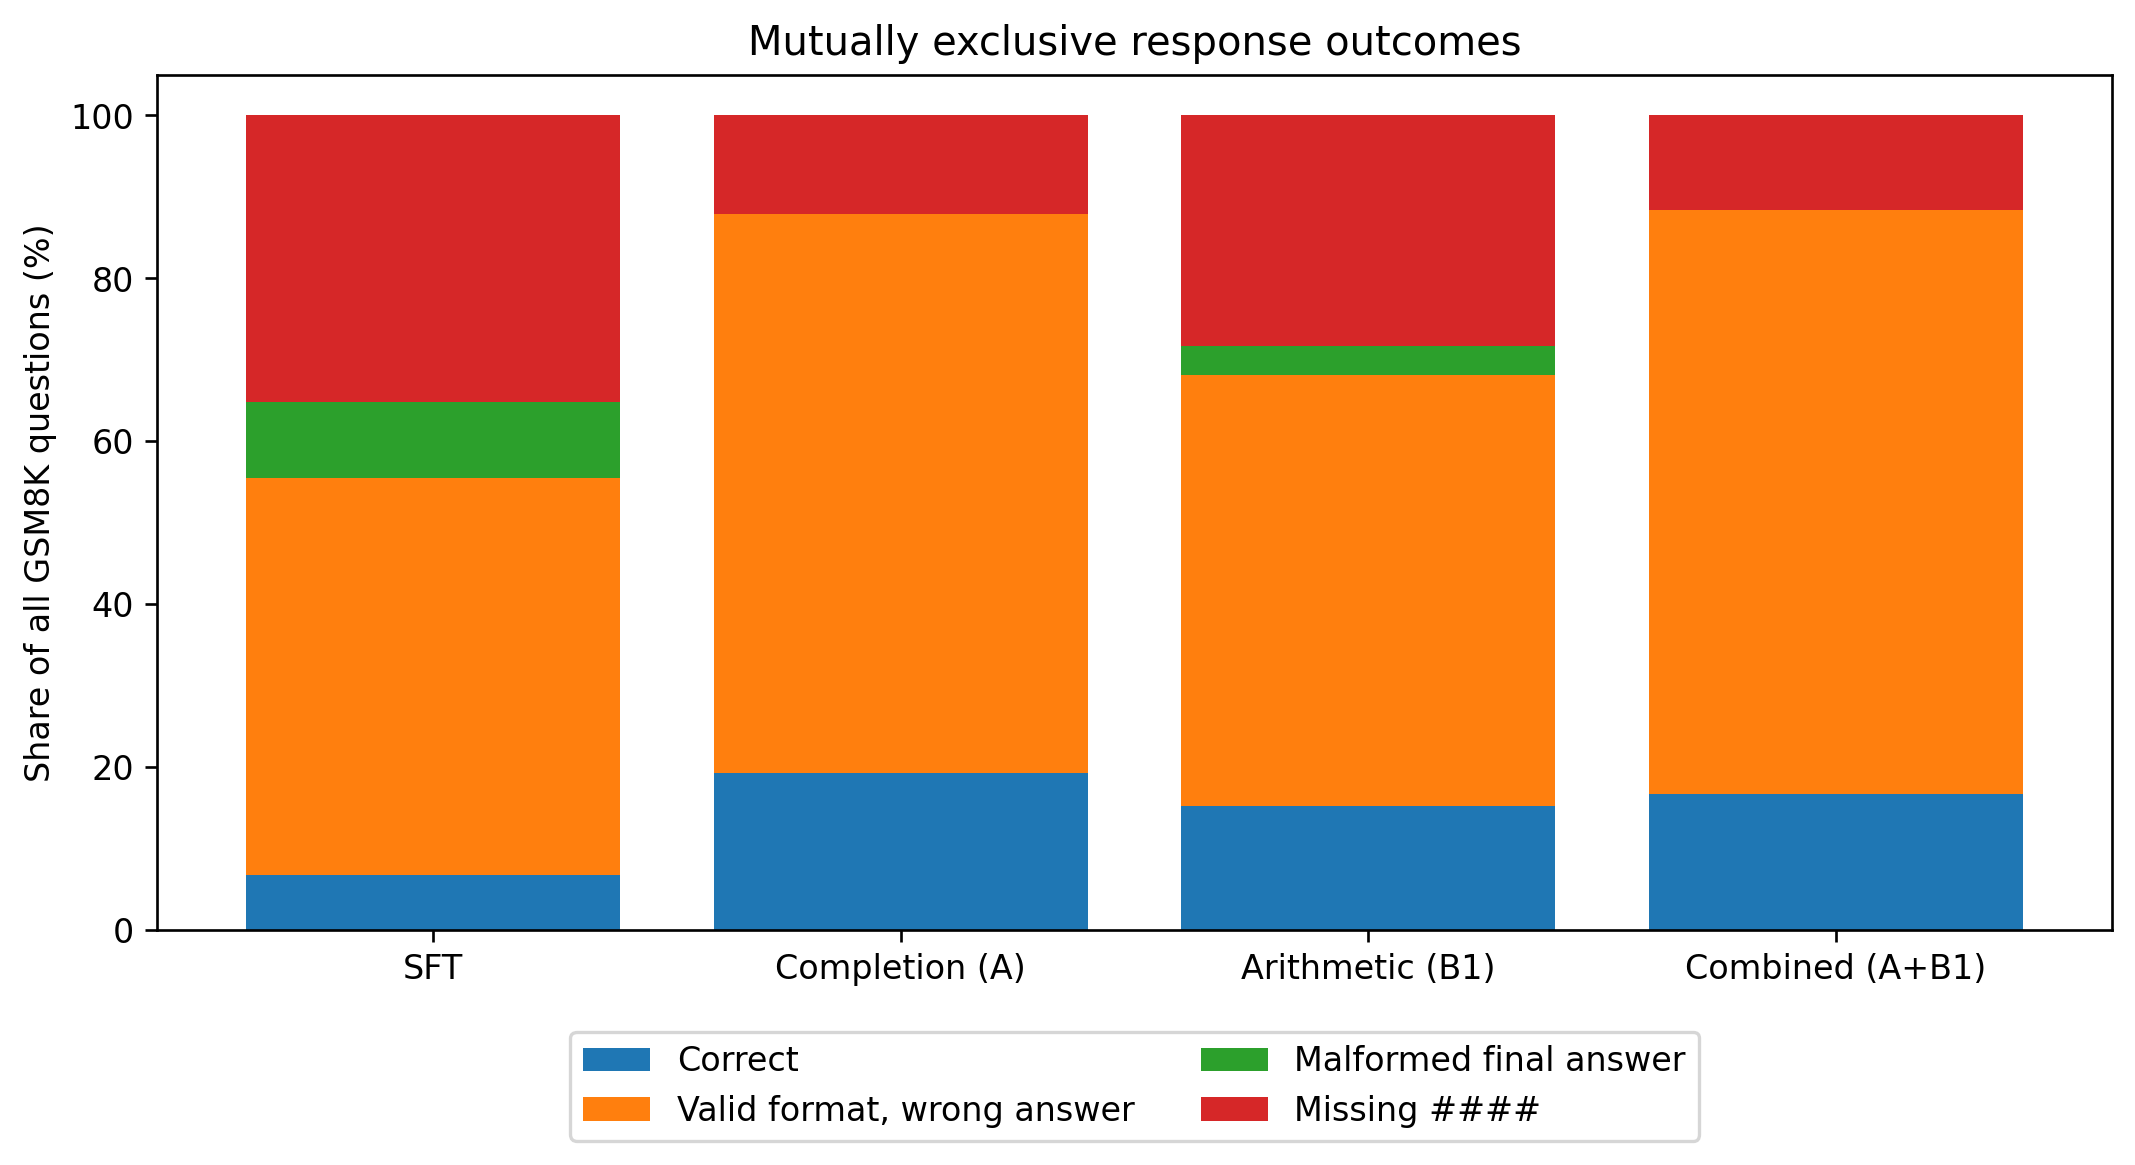
\includegraphics[width=0.84\textwidth]{figures/p4_response_outcomes.png}
\caption{Correct and incorrect test responses grouped by final-answer format. Both the completion and combined rewards greatly reduce missing and malformed final answers, but the combined model produces more well-formatted wrong answers.}
\label{fig:p4_failures}
\end{figure}

\begin{figure}[h]
\centering
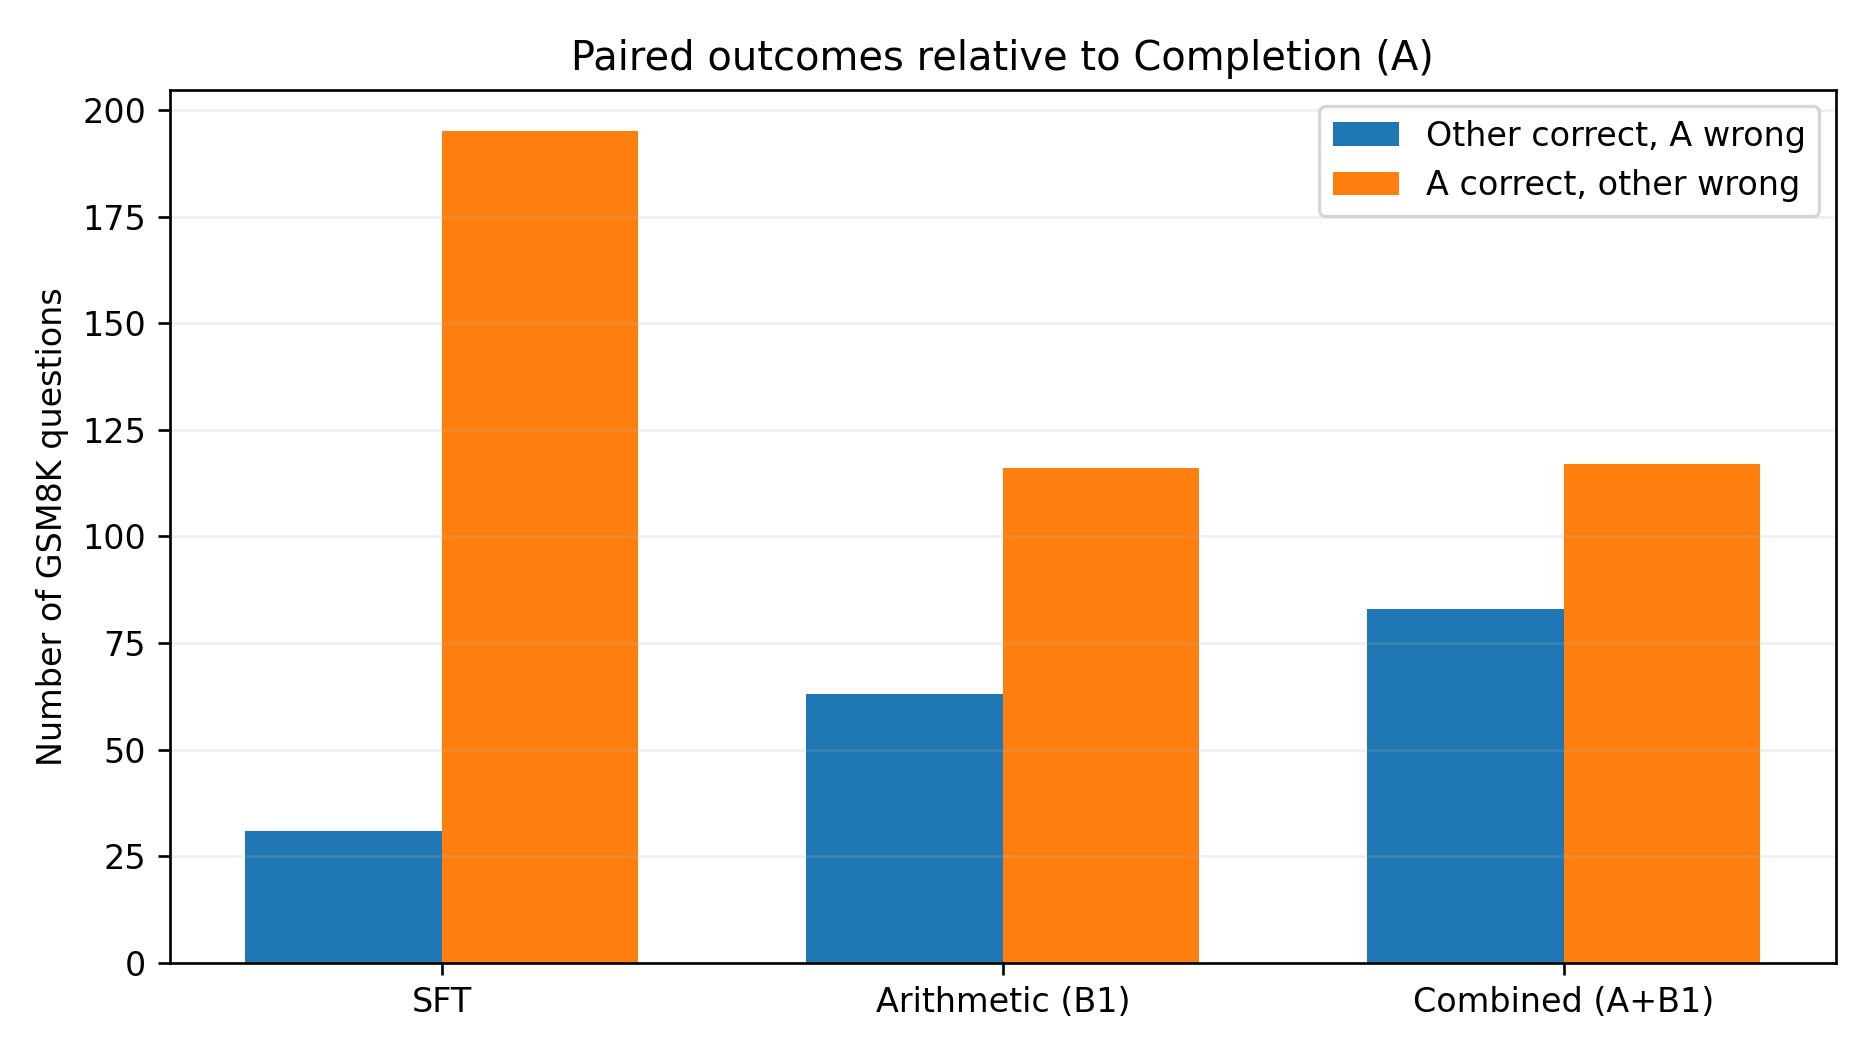
\includegraphics[width=0.82\textwidth]{figures/p4_pairwise_flips.png}
\caption{Question-level gains and losses relative to completion-only, matched by GSM8K question index. The gains and losses are not symmetric even when two models have similar overall accuracy.}
\label{fig:p4_flips}
\end{figure}

Completion-only reduces missing markers from 465 for SFT to 160, and combined reduces them to 154. In contrast, arithmetic-only still has 374 missing markers and 47 malformed final lines. This is consistent with the first reward targeting answer completion directly. Combined produces slightly more well-formed responses than completion (1{,}165 against 1{,}159 under our strict parser), but it also produces more well-formed wrong answers (946 against 906). The combined bonus therefore improves the visible format without yielding the best mathematical accuracy.

For a concrete example, on the question ``An eraser costs \$2 and a pencil costs \$3. How much do 6 erasers and 8 pencils cost?'', completion-only correctly computes $6(2)+8(3)=36$ and ends with \code{\#\#\#\# 36}. Arithmetic-only stops after ``An eraser costs \$2'', without giving a final answer. This illustrates the kind of failure the completion bonus addresses, although a single example does not establish why the models differ.

\textbf{Interpretation and limits.} The results suggest that getting this small model to finish in the scorer's expected format is a more useful intervention than adding our strict reference-matched arithmetic reward. This does not show that intermediate reasoning rewards are generally ineffective: equivalent but differently written calculations receive no arithmetic bonus here, and we tested only one weight, one random training run per method, and one model size. The original correctness-only run's interrupted optimizer trajectory is an additional limitation. Our strongest result under these conditions is completion-only reward shaping, raising greedy test accuracy from the historical 14.71\% to 19.18\%.


\section*{Part 5: On-policy distillation}

\subsection*{Method and pre-committed hypothesis}
We implemented a version of the fixed-teacher on-policy distillation method described by Thinking Machines Lab \cite{onpolicydistill}. Unlike supervised fine-tuning on teacher-generated answers, the student generates its \emph{own} GSM8K responses, and a frozen teacher scores the same generated tokens. This lets the teacher give token-level feedback even when the student's final numerical answer is wrong. We chose this approach rather than Self-Distillation Policy Optimization (SDPO) \cite{sdpo}, which constructs a feedback-conditioned self-teacher; our setup uses a separate, already trained RL checkpoint as the teacher. The hypothesis was committed before the experiment in \code{a4/PART5\_HYPOTHESIS.md} (PR \#44): denser on-policy token feedback might improve greedy GSM8K accuracy relative to the SFT starting point and correctness-only RL, or reach comparable accuracy with fewer updates. We also anticipated that the teacher's limited quality could prevent an improvement.

\textbf{Objective.} For student-sampled token $y_t$ given the preceding trajectory $h_t$, let $p_\theta(y_t\mid h_t)$ be the student probability and $q(y_t\mid h_t)$ the frozen teacher probability. Our per-token reverse-KL policy-gradient estimator uses the detached advantage
\[
A_t=\mathrm{stopgrad}\!\left(\log q(y_t\mid h_t)-\log p_\theta(y_t\mid h_t)\right),
\qquad
L=-\frac{1}{N}\sum_{t\in\mathcal V}\log p_\theta(y_t\mid h_t)\,A_t,
\]
where $\mathcal V$ contains valid student-generated tokens and $N=|\mathcal V|$. The teacher forward pass has no gradients; prompts, padding and forced tool tokens are masked. This is a sampled, zero-discount gradient estimator, not an exact full-vocabulary KL. We log the sampled difference $\log p_\theta-\log q$ as a diagnostic. The original GSM8K binary correctness reward is logged but \emph{not} used to update the student. Implementation and tests are in \code{a4/part5\_distillation.py} and \code{a4/nanochat/scripts/chat\_distill.py} (PR \#45); PR \#47 adds explicit checkpoint recovery after preemption.

\subsection*{Setup and ablations}
The student starts from our default SFT checkpoint at step 466. The frozen teacher is the completion-reward RL model from Part 4, also at step 466 (19.18\% GSM8K test accuracy). We used the GSM8K training split for optimization, one epoch (467 optimizer steps), 16 questions and 16 sampled student responses per step, temperature 1, top-$k$ 50, and eight H100 GPUs. The main run allowed at most 256 new tokens per response and used an initial learning-rate fraction of 0.05, followed by the same linear learning-rate rampdown as nanochat's RL script. Pass@$k$ was evaluated every 60 steps on 400 test questions using sampled decoding; all final results below come from a separate greedy, 512-token evaluation of the full 1{,}319-question test set. Training runs were logged to Weights \& Biases (\code{nanochat-distill}).

After the main experiment showed many responses without a final answer, we chose two exploratory ablations. \textbf{Lower learning rate} changes only the initial LR fraction, from 0.05 to 0.01. \textbf{Shorter rollouts} changes only the maximum \emph{training} response length, from 256 to 128 tokens; test-time decoding remains at 512 tokens. Both otherwise use the same student initialization, teacher, data, optimizer settings and 467-step target. We did not use an extra final-answer reward in either distillation run. These choices were made after observing the main run, not pre-registered with the original hypothesis.

\textbf{Interruption.} The lower-LR run was preempted by Modal after step 239. Its last durable checkpoint was step 180, so we resumed from that checkpoint for steps 181--466, saving the continuation under a new run name (\code{a4-p5-distill-low-lr-resume-v1}). The checkpoints do not contain optimizer state; the resumed optimizer was reinitialized. Thus this is a useful ablation of the LR setting but not an exactly matched, uninterrupted training trajectory. The main and shorter-rollout runs completed without this particular interruption.

\subsection*{Results}
Table~\ref{tab:p5} summarizes the full-test results. Main distillation improved on SFT (8.79\% against 6.75\%), but fell behind both the Part 3 correctness-only RL model (14.71\%) and the Part 4 completion-reward teacher (19.18\%). Both ablations recovered roughly five percentage points: 13.72\% for lower LR and 14.03\% for shorter rollouts. Neither surpassed the RL baselines. The four-question difference between the ablations is not meaningful on its own.

\begin{table}[h]
\centering
\small
\begin{tabular}{lrrr}
\toprule
Model & Correct / 1{,}319 & Accuracy (\%) & Change vs. main distill. \\
\midrule
SFT starting model & 89 & 6.75 & $-2.05$ pp \\
Main distillation, 256 tokens & 116 & 8.79 & -- \\
Lower LR, 0.01 (resumed) & 181 & 13.72 & $+4.93$ pp \\
Short rollouts, 128 tokens & \textbf{185} & \textbf{14.03} & \textbf{$+5.23$ pp} \\
Correctness-only RL (Part 3) & 194 & 14.71 & $+5.91$ pp \\
Completion RL teacher (Part 4) & 253 & 19.18 & $+10.39$ pp \\
\bottomrule
\end{tabular}
\caption{Greedy GSM8K accuracy on all 1{,}319 test problems, with up to 512 generated tokens. The Part 3 RL result is historical; the lower-LR student was interrupted and resumed without optimizer state. All percentage-point changes use the main distillation model as reference.}
\label{tab:p5}
\end{table}

\begin{figure}[h]
\centering
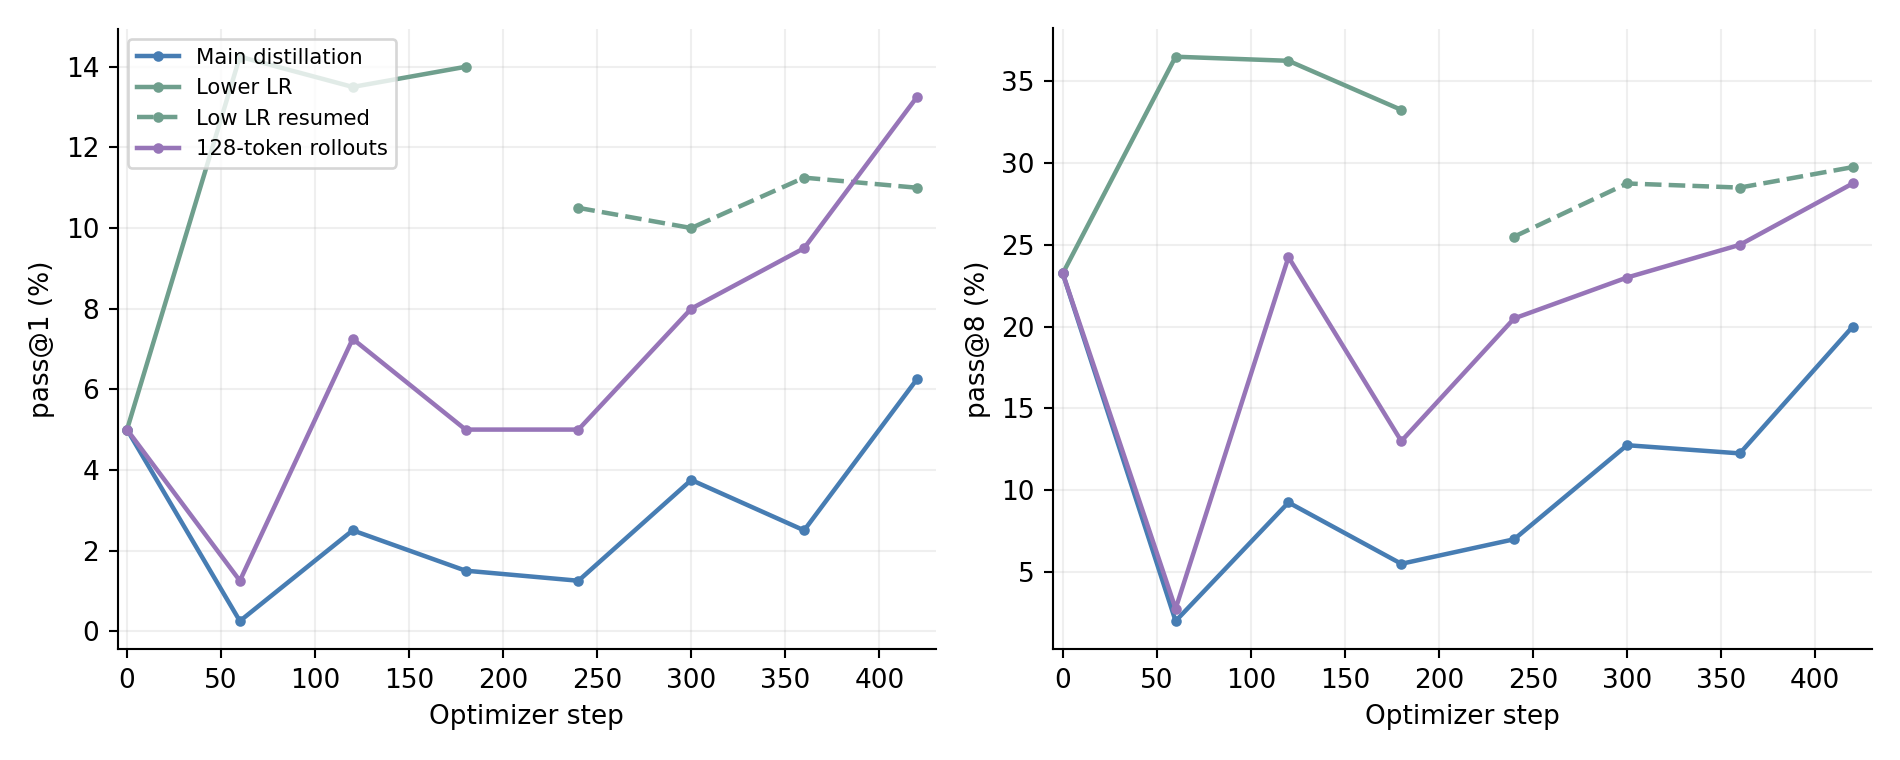
\includegraphics[width=0.88\textwidth]{figures/p5_training_passk.png}
\caption{Sampled GSM8K pass@1 (left) and pass@8 (right) on 400 test questions during training. The low-LR curve combines its original run (solid) and resumed segment (dashed); the join includes an optimizer reset. These sampled metrics differ from the greedy full-test results in Table~\ref{tab:p5}.}
\label{fig:p5_passk}
\end{figure}

\textbf{Training behavior.} The main run's pass@1 fell from 5.0\% at step 0 to 0.25\% at step 60, then recovered to 6.25\% at the last periodic evaluation (step 420). Its sampled reverse-KL diagnostic fell from about 0.593 to 0.038, while its mean logged sequence length fell from about 215 to 113 tokens. The shorter-rollout run finished with sampled pass@1 of 13.25\% at step 420; the lower-LR continuation finished with 11.0\%. A smaller sampled KL did not by itself imply high test accuracy: the main run's sampled KL decreased substantially even as its test accuracy stayed well below that of the teacher. The sequence-length metric includes prompt tokens, so it should not be read as the number of generated reasoning tokens.

\textbf{Paired comparisons.} Because all four Part 5/teacher response files contain answers for the same 1{,}319 indexed questions, we can count which problems were gained and lost. Lower LR solves 103 problems missed by main distillation and loses 38 it previously solved; shorter rollouts gain 102 and lose 33. The improvements over the main run are $+4.93$ percentage points (paired question-bootstrap 95\% interval 3.18--6.67) and $+5.23$ points (3.56--6.97). Comparing the two ablations directly, shorter rollouts gain 65 and lose 61 problems against lower LR, a difference of just $+0.30$ points (95\% interval $-1.36$ to 1.97). We used 12{,}000 bootstrap resamples of test questions; these intervals quantify uncertainty across questions, \emph{not} different random training seeds or the effect of preemption.

\subsection*{What went wrong and what the ablations changed}
The main distilled student often stops without the required \code{\#\#\#\# N} final line: this occurs on 811 of 1{,}319 test questions (61.5\%), compared with 160 (12.1\%) for its RL teacher. The lower-LR and shorter-rollout models reduce missing markers to 478 (36.2\%) and 487 (36.9\%), respectively (Figure~\ref{fig:p5_outcomes}). They also raise the number of correct responses from 116 to 181 and 185. On the question where Kira buys 3 apples, 5 bananas and 6 oranges and Lola eats two fruits, the main distilled model correctly totals 14 fruits but ends after ``Lola ate 2''; both ablations complete the subtraction and report \code{\#\#\#\# 12}. This illustrates an observable completion failure, not proof of its internal cause.

\begin{figure}[h]
\centering
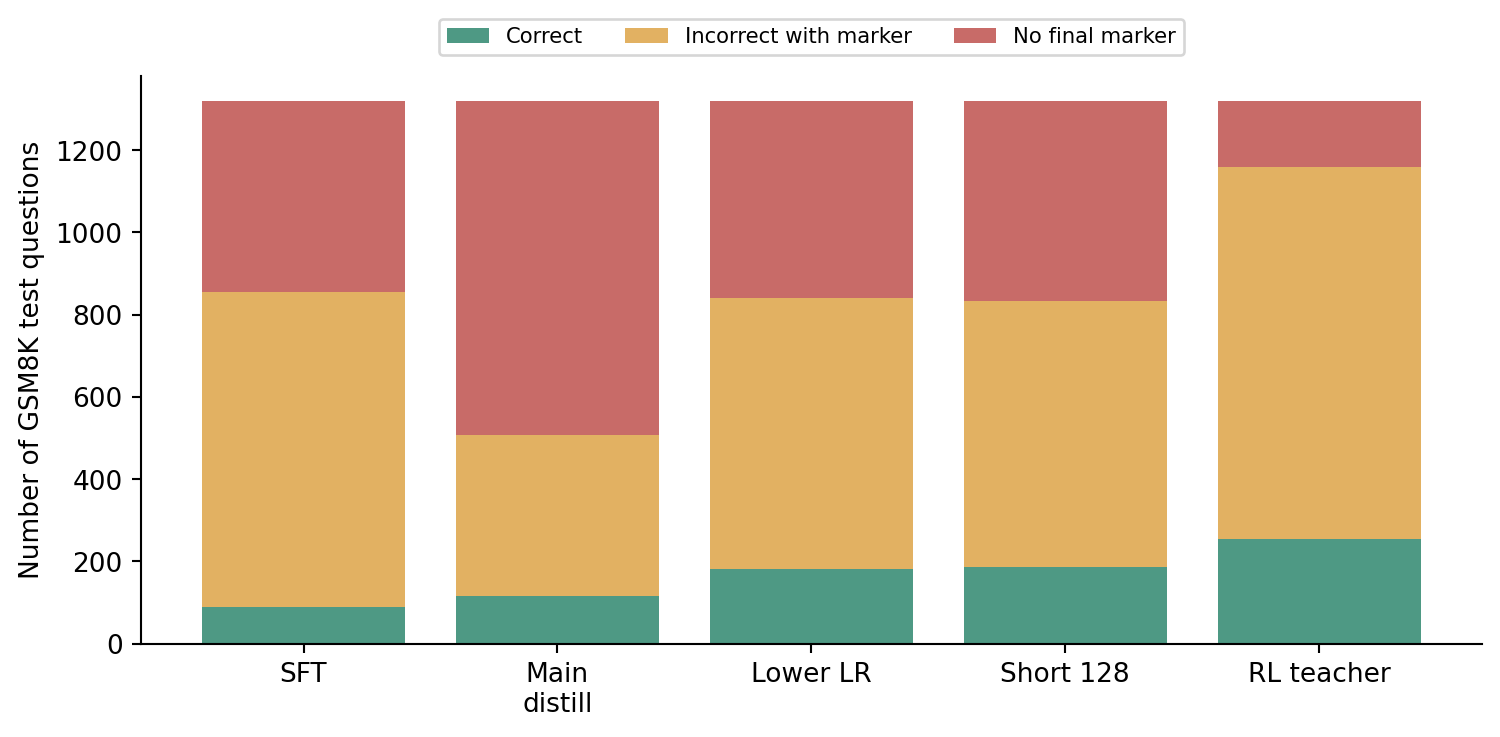
\includegraphics[width=0.88\textwidth]{figures/p5_response_outcomes.png}
\caption{Response outcomes on the same 1{,}319 held-out GSM8K problems. ``No final marker'' means the literal \code{\#\#\#\#} does not appear in the generated response. The incorrect-with-marker category includes malformed or wrong final answers.}
\label{fig:p5_outcomes}
\end{figure}

The results are consistent with a failure to retain answer-completion behavior during the original distillation optimization, though the saved responses cannot identify its cause. The lower learning rate may preserve the starting policy better, and the shorter-rollout training may change the distribution of trajectories on which the teacher supplies feedback. Neither explanation is isolated conclusively: the low-LR run restarted its optimizer, and we have only one training run per configuration. Shorter rollouts also alter the training-token budget, so their effect cannot be attributed solely to improved reasoning or efficiency.

\textbf{Comparison with RL.} Correctness-only RL directly rewards solving a complete problem; our distillation objective instead matches a frozen teacher's token probabilities on student-generated trajectories. That supervision is denser, but it does not explicitly reward finishing the numerical answer. In this small-model setting, the main distillation student achieved only 8.79\%, against 14.71\% for correctness-only RL and 19.18\% for its teacher. Even the stronger ablations remained below both: 13.72\% and 14.03\%. Our initial hypothesis was therefore only partly supported: distillation improved on SFT, but did not outperform RL or show better sample efficiency at the measured checkpoints. The most useful result is that the training configuration strongly affects whether dense teacher feedback translates into correct, completed answers. This comparison is limited by single runs, the resumed low-LR optimizer, the different reward objectives and the teacher's own errors.


\section*{Reproducing our work}
All code is in PRs \#34--\#45 and \#47 on the course repository
(cache, launcher, extra data, evaluation tools, RL rewards,
distillation, checkpoint recovery, and analysis).
The commands are in \code{a4/modal\_launch.py}'s header,
for example \code{modal run a4/modal\_launch.py --script sft
--mode full --run a4-sft-default}.
Figures are made by \code{a4/report/make\_figures.py}
and the analysis by \code{a4/analyze\_rl.py}.
The blind-labeling check can be reproduced with
\code{a4/report/label\_check/agreement.py},
and the control data is built by
\code{a4/prepare\_control\_data.py}.

\textbf{Weights \& Biases runs.} For the Part 3 RL runs, W\&B's default x-axis counts logging calls rather than optimizer steps (W\&B step 121 corresponds to training step 60, and step 723 to training step 420). We checked pass@6, pass@7 and pass@8 against the recorded evaluation values in \code{a4/rl\_eval\_curves.json},
and they match.

For Parts 4 and 5, we logged each reward configuration and
distillation ablation separately in W\&B, tracking training
rewards or losses, sampled pass@1 and pass@8, and response
lengths. All runs used the same periodic evaluation setup
(400 GSM8K test questions every 60 optimizer steps), while
final accuracy was measured separately using greedy decoding
on all 1,319 test questions. Part 4 compares completion,
arithmetic, and combined rewards against the original RL
baseline. Part 5 compares the main distillation run against
lower-learning-rate and shorter-rollout ablations. The
lower-learning-rate run was preempted and resumed from step
180 without optimizer state, so its training history spans
two W\&B runs.

\begin{itemize}\itemsep0pt\footnotesize
\item SFT: \url{https://wandb.ai/allaith2004-university-of-toronto/nanochat-sft/runs/4qh55nxr}
\item SFT, default settings rerun on an H100: \url{https://wandb.ai/allaith2004-university-of-toronto/nanochat-sft/runs/2o3qfmwv}
\item SFT, second run of the default settings: \url{https://wandb.ai/allaith2004-university-of-toronto/nanochat-sft/runs/hqhs4e4f}
\item SFT with extra data: \url{https://wandb.ai/allaith2004-university-of-toronto/nanochat-sft/runs/jwz57oeh}
\item Midtraining: \url{https://wandb.ai/allaith2004-university-of-toronto/nanochat-mid/runs/ch85x0el}
\item Midtraining with extra data: \url{https://wandb.ai/allaith2004-university-of-toronto/nanochat-mid/runs/92v487r5}
\item RL, steps 0--60: \url{https://wandb.ai/allaith2004-university-of-toronto/nanochat-rl/runs/ktg7otwf}
\item RL, steps 61--466: \url{https://wandb.ai/allaith2004-university-of-toronto/nanochat-rl/runs/wjbcsvd1}
% Part 4: Reward-shaping experiments
\item RL, completion reward:
\url{https://wandb.ai/royceluo1216-university-of-toronto/nanochat-rl}

\item RL, arithmetic reward:
\code{a4-p4-arithmetic-v1}
(\url{https://wandb.ai/royceluo1216-university-of-toronto/nanochat-rl})

\item RL, combined rewards:
\code{a4-p4-combined-v1}
(\url{https://wandb.ai/royceluo1216-university-of-toronto/nanochat-rl})

% Part 5: On-policy distillation
\item Distillation, main:
\code{a4-p5-distill-completion-v1}
(\url{https://wandb.ai/royceluo1216-university-of-toronto/nanochat-distill})

\item Distillation, lower LR:
\code{a4-p5-distill-low-lr-v1},
resumed as
\url{https://wandb.ai/royceluo1216-university-of-toronto/nanochat-distill/runs/99ed489p}

\item Distillation, 128-token rollouts:
\code{a4-p5-distill-short128-v1}
(\url{https://wandb.ai/royceluo1216-university-of-toronto/nanochat-distill})
\end{itemize}

\begin{thebibliography}{9}\small
\bibitem{shao2024} Z.\ Shao, P.\ Wang, Q.\ Zhu, et al. DeepSeekMath: Pushing the Limits of Mathematical Reasoning in Open Language Models. arXiv:2402.03300, 2024.
\bibitem{yu2025dapo} Q.\ Yu, Z.\ Zhang, R.\ Zhu, et al. DAPO: An Open-Source LLM Reinforcement Learning System at Scale. arXiv:2503.14476, 2025.
\bibitem{liu2025} Z.\ Liu, C.\ Chen, W.\ Li, et al. Understanding R1-Zero-Like Training: A Critical Perspective. arXiv:2503.20783, 2025.
\bibitem{nanochat} A.\ Karpathy. nanochat. \url{https://github.com/karpathy/nanochat}, 2025 (announcement post: \url{https://github.com/karpathy/nanochat/discussions/1}).
\bibitem{cobbe2021} K.\ Cobbe, V.\ Kosaraju, M.\ Bavarian, et al. Training Verifiers to Solve Math Word Problems. arXiv:2110.14168, 2021.
\bibitem{metamath} L.\ Yu, W.\ Jiang, H.\ Shi, et al. MetaMath: Bootstrap Your Own Mathematical Questions for Large Language Models. arXiv:2309.12284, 2023.
\bibitem{orcamath} A.\ Mitra, H.\ Khanpour, C.\ Rosset, A.\ Awadallah. Orca-Math: Unlocking the Potential of SLMs in Grade School Math. arXiv:2402.14830, 2024.
\bibitem{fox} Z.\ Lin, E.\ Nikishin, X.\ O.\ He, A.\ Courville. Forgetting Transformer: Softmax Attention with a Forget Gate. arXiv:2503.02130, 2025.
\bibitem{onpolicydistill}
Thinking Machines Lab.
On-Policy Distillation, 2025.
\url{https://thinkingmachines.ai/blog/on-policy-distillation/}

\bibitem{sdpo}
J. H\"ubotter et al.
Reinforcement Learning via Self-Distillation, 2026.
arXiv:2601.20802.
\end{thebibliography}

\end{document}
